\section{Methodology}
\label{sec:method}

\subsection{Overall Framework of the Proposed MAFF-Net}

Accurate delineation of the lesion region in dermoscopy is a prerequisite for downstream tasks such as morphological assessment, malignancy scoring, and treatment planning, yet manual delineation is time-consuming and varies between observers, which motivates reliable automated segmentation. The task remains difficult because dermoscopic images frequently exhibit low contrast between lesion and surrounding skin, gradual or ill-defined boundaries, occlusion by hair and vascular structures, and pronounced variability in lesion shape, scale, and pigmentation. Methods intended for clinical support must therefore remain robust under these conditions and, in particular, must recover lesion boundaries faithfully.

Large-scale visual foundation models supply transferable representations that reduce the dependence on scarce annotated medical data, but their direct application to dermoscopy is limited by the domain gap between natural and medical images. The Original MAFF-Net \cite{ref15} addresses this gap by adapting a pretrained foundation backbone with multi-scale perception adaptation (MMPA) and frequency-guided feature fusion (FGFF), and by regularising the decoder through an auxiliary Reconstruction Decoder Branch (RDB). This design integrates spatial and spectral information effectively but does not explicitly separate the spatial and frequency representations prior to fusion, which motivates an explicit dual-stream integration in which the two domains are treated as separate, reconciled streams.

Accordingly, this work pursues a targeted refinement of the MAFF-Net framework rather than its replacement: the validated components of the Original MAFF-Net are retained and only the fusion pathway is redesigned, where explicit dual-stream integration is justified. The frozen encoder, the convolutional decoder, and the auxiliary reconstruction branch are preserved without alteration, so that the transferable priors and the proven decoding pathway continue to anchor the network. In place of the original single fusion pathway, the multi-scale features produced by the encoder are processed along two parallel routes: a spatial stream that preserves regional and contextual structure, and a frequency stream that emphasises boundary-sensitive detail. Fig.~\ref{fig:architecture} presents the overall organisation of the Proposed MAFF-Net, in which the two streams are reconciled and combined into a unified representation before decoding.

\begin{figure*}[!t]
\centering
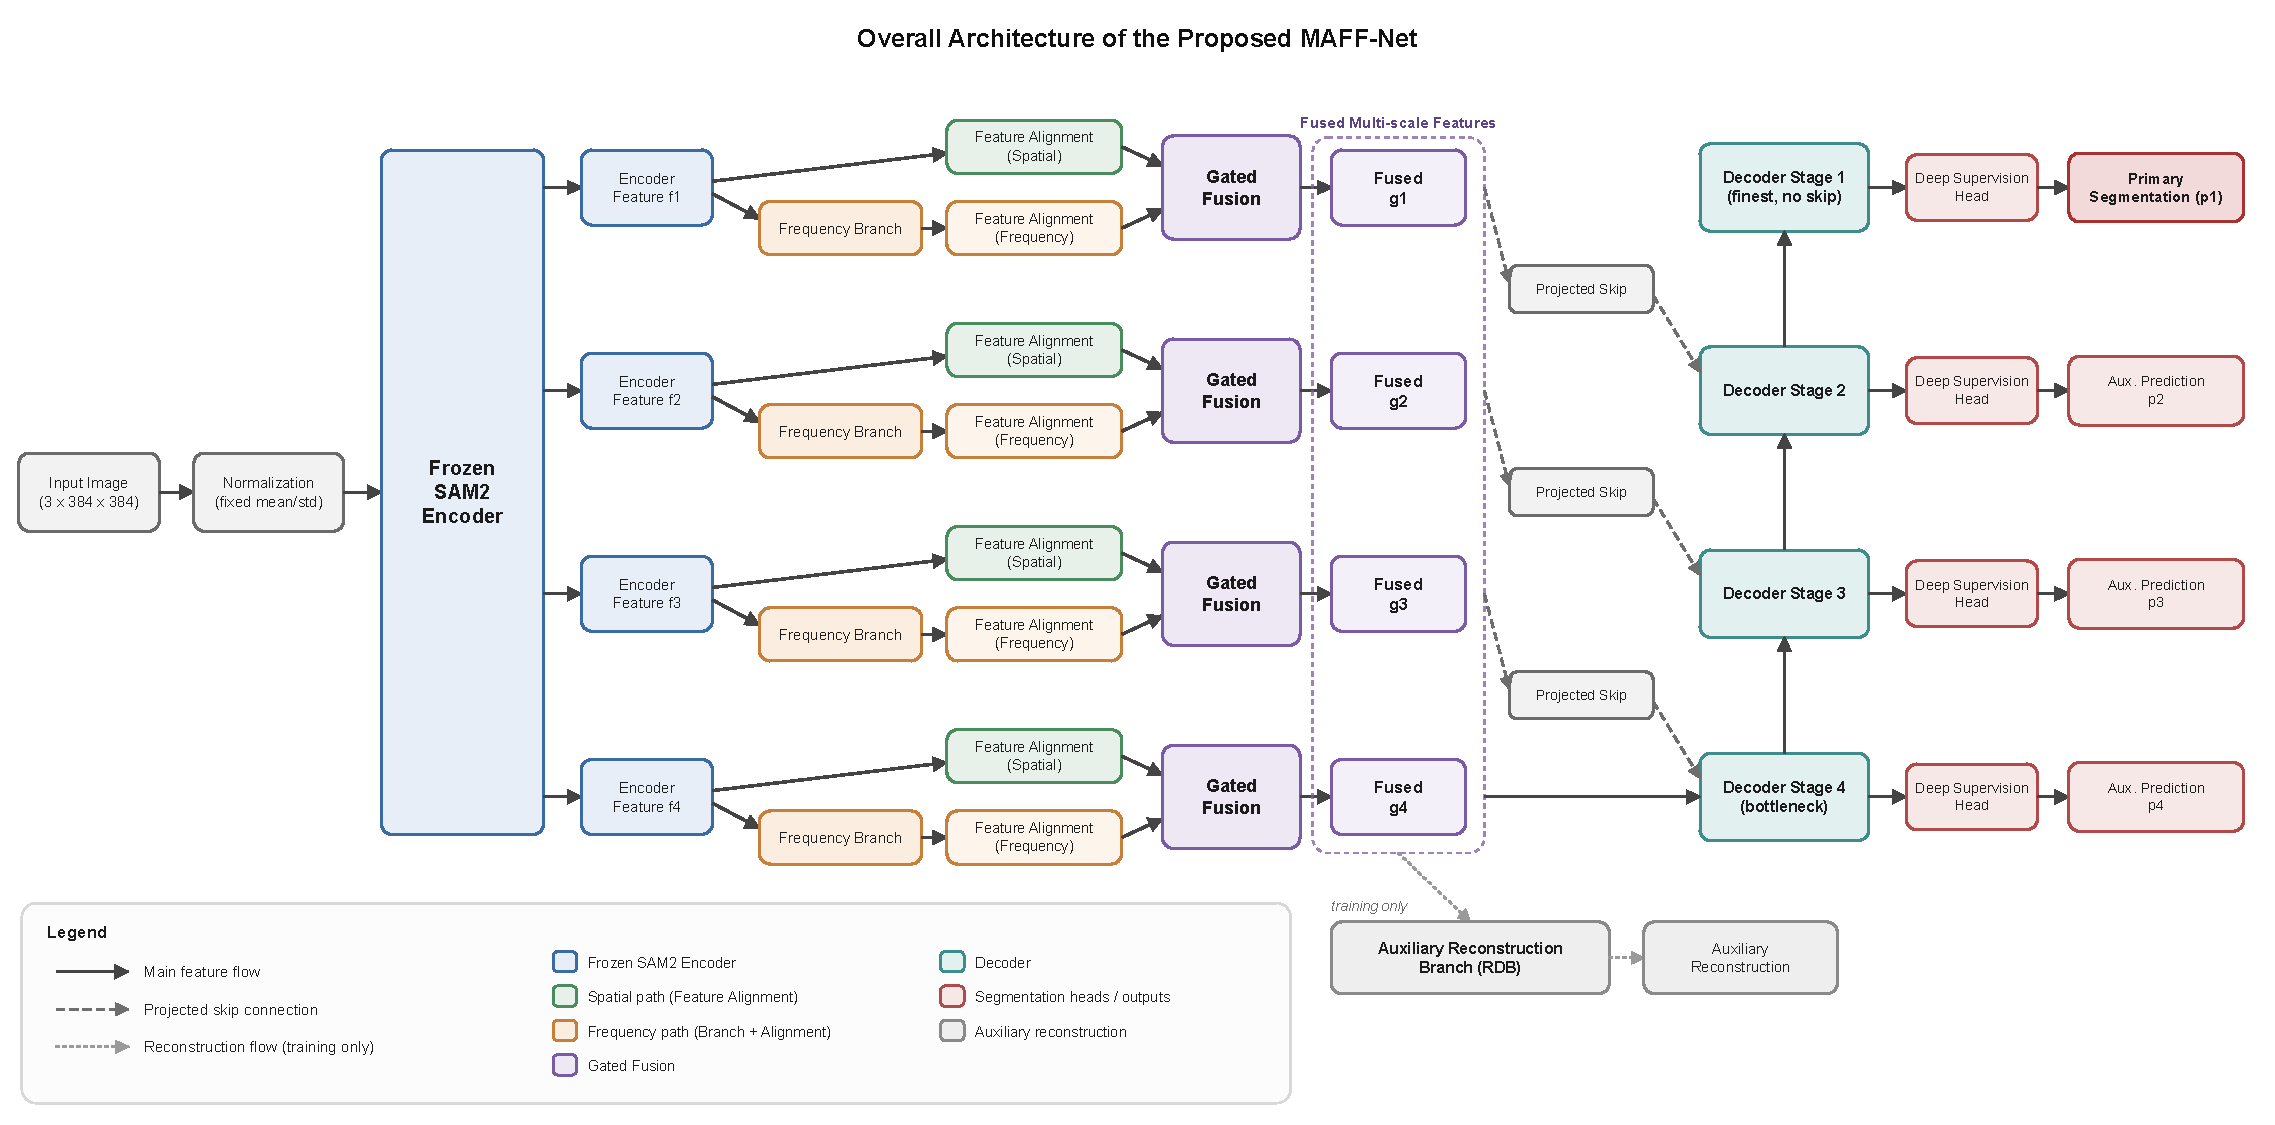
\includegraphics[width=\textwidth]{Figure1_Architecture.pdf}
\caption{Overall architecture of the Proposed MAFF-Net. A frozen SAM2 encoder
produces four multi-scale features, each processed by parallel spatial and
frequency pathways whose aligned representations are combined by gated fusion.
The three shallower fused features enter the decoder through projected skip
connections and the deepest enters as the decoder bottleneck; four
deep-supervision heads produce the segmentation outputs, of which the
highest-resolution one is the primary prediction, and an auxiliary
reconstruction branch operates on the fused features during training.}
\label{fig:architecture}
\end{figure*}

The processing pipeline proceeds as follows. A dermoscopic image is passed through the frozen encoder, yielding a set of multi-scale feature representations; at each scale, the corresponding feature is routed simultaneously into the spatial and frequency streams, so that contextual and boundary-oriented information are extracted in parallel rather than entangled. The two streams are reconciled and combined into a unified representation at each scale, and these fused multi-scale representations are propagated to the convolutional decoder, which produces the lesion segmentation map. During training, the auxiliary reconstruction branch operates alongside the decoder to regularise the learned features and supervision is applied at multiple decoder stages; at inference, only the primary segmentation output is retained.

The components introduced in the fusion pathway are stated here without implementation detail. The Frequency Branch provides an explicit spectral route that emphasises boundary-related content within each encoder feature; the Feature Alignment Module harmonises the statistics of the spatial and frequency representations so that they can be combined consistently; and the Gated Fusion Module replaces implicit fusion with a learned, lightweight combination of the two aligned streams. The network is additionally trained under Boundary-aware Deep Supervision (BDS) and Edge-weighted Reconstruction (EWR), jointly referred to as Boundary-centric Dual Supervision (BcDS), which direct the optimisation toward the lesion contour. The encoder, decoder, and reconstruction branch are preserved from the Original MAFF-Net and are not claimed as contributions of this work.

Taken together, these components constitute a framework that separates spatial and spectral processing, reconciles the two domains before fusion, and reinforces boundary fidelity through BcDS while continuing to rely on the pretrained backbone. The remaining subsections describe each element in detail, beginning with the frozen encoder that produces the multi-scale features on which the two streams operate.

\subsection{Overall Network Architecture}

The Proposed MAFF-Net is a dual-stream encoder--decoder network built on a pretrained visual foundation backbone. Its guiding architectural principle is a clear separation of responsibilities: the encoder supplies transferable multi-scale representations, two parallel pathways process complementary aspects of them, a dedicated stage reconciles and combines the two pathways, and a convolutional decoder produces the segmentation output. The frozen encoder, the convolutional decoder, and the auxiliary reconstruction mechanism are preserved from the Original MAFF-Net, and the redesign is confined to the pathway responsible for combining spatial and spectral information. The network is therefore best understood as a structured composition of preserved and newly introduced components, each assigned a distinct role in the overall processing chain, rather than a monolithic model.

The complete architecture is illustrated in Fig.~\ref{fig:architecture}, which depicts the end-to-end structure of the Proposed MAFF-Net from the input dermoscopic image to the predicted segmentation map. As shown, an input image is first encoded into a set of multi-scale feature representations by the frozen encoder. Each representation is then dispatched to two parallel pathways --- a spatial pathway that retains regional and contextual structure and a frequency pathway that emphasises boundary-sensitive content --- which are reconciled by the Feature Alignment Module and merged by the Gated Fusion Module into a single fused representation at each scale. The fused representations pass to the convolutional decoder, which aggregates information across scales to yield the segmentation map, while an auxiliary reconstruction branch operates alongside the decoder as a training-time regularisation signal; it runs on every forward pass, and at inference its output is discarded and only the primary segmentation output is retained.

At the level of module organisation, the network comprises three functional groups. The first is the preserved backbone: the frozen encoder, adopted from the Original MAFF-Net, which supplies hierarchical multi-scale features and is not adapted during training. The second is the newly introduced fusion pathway, which replaces the single fusion route of the Original MAFF-Net and comprises the Frequency Branch, the Feature Alignment Module, and the Gated Fusion Module. The third comprises the preserved decoding and regularisation components: the convolutional decoder that reconstructs spatial resolution and produces the prediction, and the auxiliary reconstruction branch that constrains the learned features during training. Supervision of the network is governed by Boundary-centric Dual Supervision, which comprises Boundary-aware Deep Supervision and Edge-weighted Reconstruction.

The resulting information flow is a parallel-then-merge structure: at every scale the encoder features fan out into the two pathways so that contextual and boundary-oriented information are extracted concurrently rather than in a single entangled route, are reconciled onto a shared footing by the Feature Alignment Module, and are collapsed back into a single fused stream by the Gated Fusion Module before decoding. The convolutional decoder integrates the fused multi-scale representations from coarse to fine to recover the full-resolution map; during training, the auxiliary reconstruction branch draws on the same fused features to encourage stable and informative representations, while deep supervision at multiple decoder stages guides the intermediate predictions toward the target. In sum, the representation is split into complementary pathways, reconciled, fused, and finally decoded.

The rationale follows from the difficulties of dermoscopic segmentation. Separating the spatial and frequency pathways provides explicit access to boundary-related spectral content while retaining the contextual structure needed to localise the lesion, addressing the low contrast and ill-defined boundaries characteristic of these images. Aligning the pathways before fusion is intended to ensure that representations of different origin are combined on compatible terms, and delegating the combination to a learned gate allows the network to weigh the two domains adaptively rather than committing to a fixed rule. Retaining the pretrained backbone preserves the transferable priors that mitigate the scarcity of annotated dermoscopic data, and retaining the established decoder and reconstruction branch keeps a proven decoding pathway intact, so that the observed behaviour of the network can be attributed to the redesigned fusion pathway and the boundary-centric supervision rather than to changes in the backbone or decoder. This maintains continuity with the philosophy of the Original MAFF-Net, in which a strong frozen encoder is adapted for the medical domain rather than trained from scratch.

Having established the blueprint, the module organisation, and the information flow, the following subsections describe each component in detail --- the frozen encoder, the Frequency Branch, the Feature Alignment Module, the Gated Fusion Module, and the decoder with its auxiliary reconstruction branch --- concluding with the training objective that implements Boundary-centric Dual Supervision.

\subsection{Frozen Foundation Backbone}

Visual foundation models pretrained on large and diverse image collections provide transferable representations that are difficult to obtain from the limited annotated data available in dermoscopy. The Segment Anything Model (SAM) family \cite{ref9}, in particular, is trained at a scale that yields general-purpose spatial priors, and the Original MAFF-Net showed that such a model can be adapted to skin-lesion segmentation by retaining its image encoder as a fixed feature extractor rather than training a network from scratch. Preserving a pretrained backbone in this manner offers two practical advantages that are especially relevant in the medical setting: it transfers robust representations learned from abundant natural images, and it avoids the risk of overfitting and the substantial cost of updating a very large encoder on a comparatively small medical dataset. The Proposed MAFF-Net preserves this design choice without alteration; the SAM2 image encoder \cite{ref10} is adopted from the Original MAFF-Net and used as the feature-extraction foundation of the network.

Within the architecture, the backbone maps the input dermoscopic image, standardised to the statistics expected by the encoder, into a set of intermediate feature representations. Its parameters are frozen throughout training --- neither updated by the optimisation process nor otherwise modified in this work --- so the trainable capacity of the network is concentrated entirely in the modules that operate downstream of it, and the representations it produces remain stable and consistent across training. The encoder is thus used exactly as provided, and none of the contributions claimed in this paper reside within it.

A property important for lesion segmentation is that the backbone is hierarchical, producing representations at several spatial resolutions and semantic levels rather than a single feature map: the shallower representations retain fine spatial detail and are informative about local structure, whereas the deeper ones encode coarser, more semantic context describing the lesion as a whole. This range of scales is well suited to dermoscopic images, in which lesions vary considerably in size and in which accurate delineation requires both localisation of the overall lesion region and sensitivity to fine boundary structure. By spanning these scales, the frozen encoder supplies the multi-scale information on which the subsequent scale-adaptive processing depends, and it does so uniformly for every input without any scale-specific tuning.

These multi-scale representations are the common input to all downstream components of the Proposed MAFF-Net, and it is at this point that the contributions of the present work begin. Each representation is routed into the two parallel pathways, aligned, and combined before decoding, so that the spatial pathway, the Frequency Branch, the Feature Alignment Module, and the Gated Fusion Module all operate on the encoder outputs rather than on the raw image. Redesigning or fine-tuning the backbone is unnecessary for the goals of this study, because the limitation motivating the proposed modules concerns how spatial and spectral information are combined after extraction, not the quality or availability of the extracted features themselves; keeping the encoder fixed also ensures that any change in segmentation behaviour can be attributed to the redesigned fusion pathway and its supervision rather than to the feature extractor. Having established the role of the encoder and the multi-scale representations it provides, the following subsection describes the Frequency Branch, the first of the newly introduced modules, which derives a boundary-sensitive spectral representation from each encoder feature.

\subsection{Frequency Branch for Boundary-Aware Spectral Representation}

Boundary-related information is predominantly represented within the higher-frequency components of an image. Repeated downsampling in convolutional encoder hierarchies reduces the prominence of fine spatial detail while emphasising higher-level semantic information, so that the edge structure associated with the boundary becomes less prominent in the deeper representations than the coarser content describing the lesion interior. This is compounded by the low contrast typical of dermoscopy, where the small intensity difference between lesion and surrounding skin makes spatial gradients weak and often unreliable indicators of the true boundary. The frequency domain offers a complementary view in which higher-frequency edge structure and lower-frequency background can be separated more explicitly than in a single spatial representation. These observations motivate the Frequency Branch, which provides the Proposed MAFF-Net with an explicit spectral route dedicated to boundary-sensitive content.

The Frequency Branch is a parameter-free spectral module, instantiated independently at each encoder scale so that a dedicated spectral representation is derived at every level of the hierarchical feature set. It retains the high-frequency components of an incoming feature while suppressing the low-frequency components by means of a radial high-pass filter, whose single cutoff --- the radial boundary between the suppressed and retained frequencies --- is a fixed hyperparameter rather than a learned quantity. The module therefore contains no trainable parameters and adds nothing to the learnable capacity of the network, acting as a fixed, interpretable operator whose behaviour is fully determined by that cutoff, and its output constitutes the boundary-aware spectral representation from which the module takes its purpose. As one of the newly introduced components of this work, the Frequency Branch is illustrated schematically in Fig.~\ref{fig:freqbranch}.

\begin{figure}[!t]
\centering
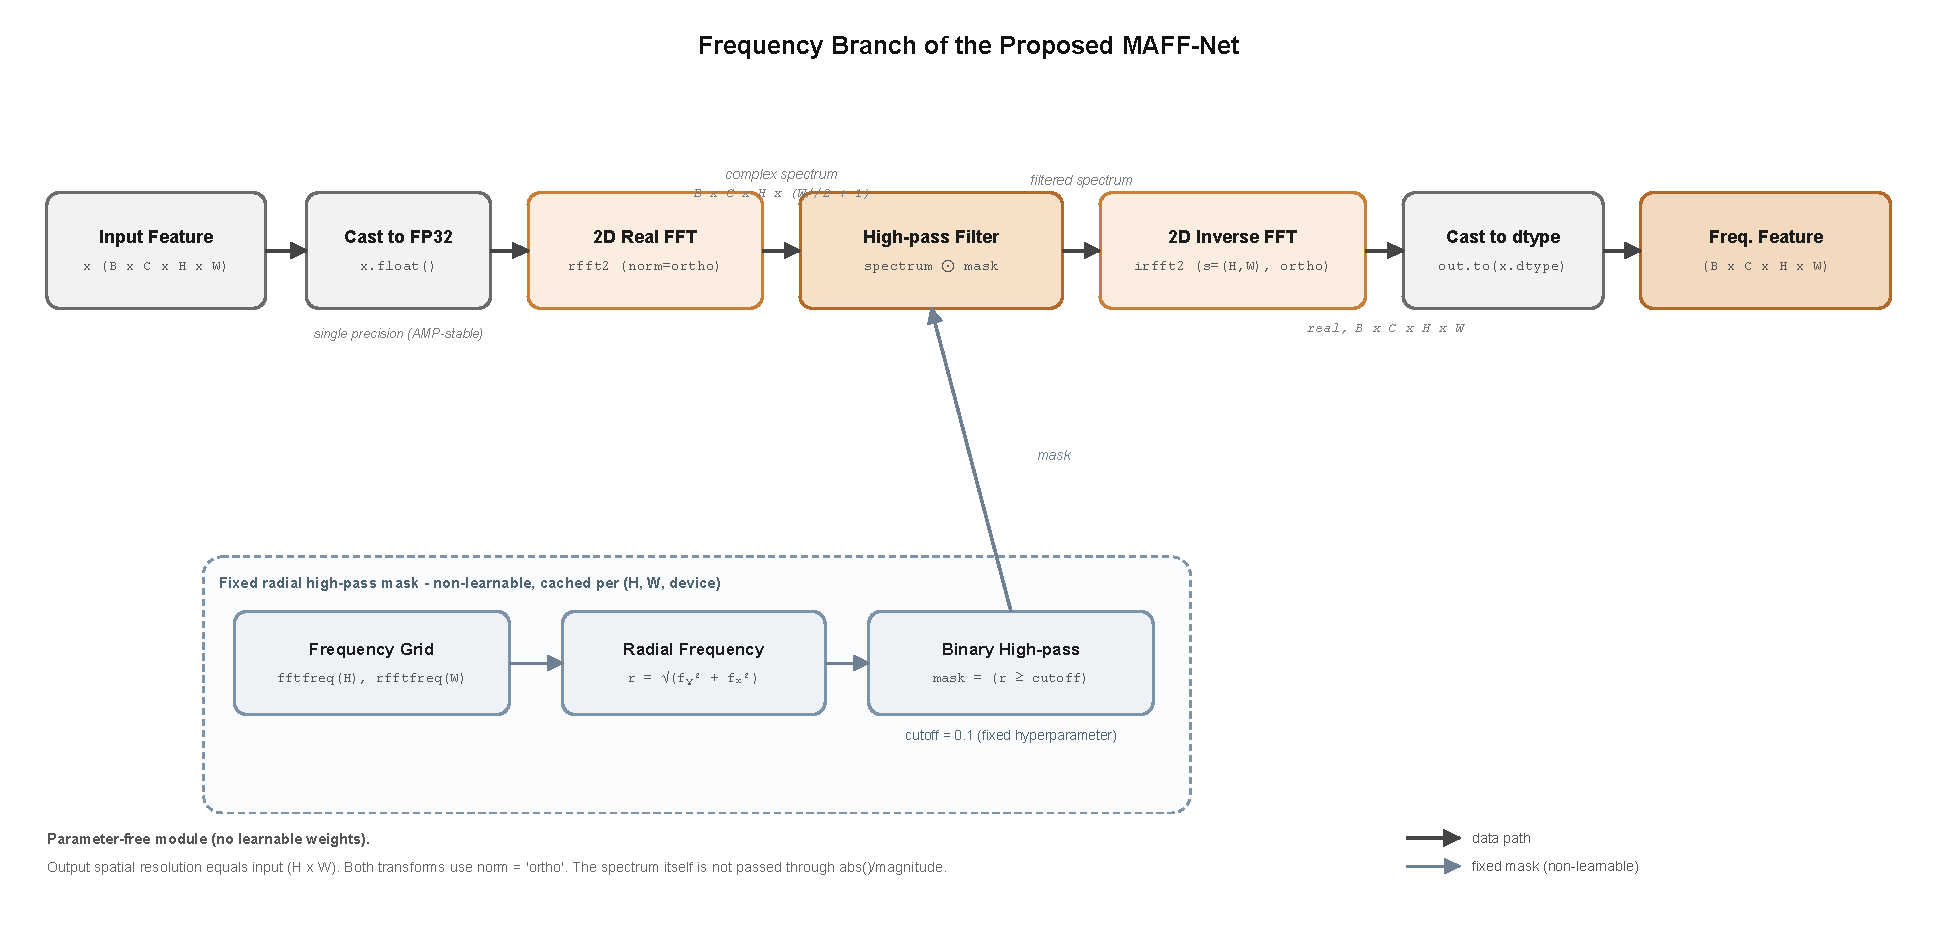
\includegraphics[width=\columnwidth]{Figure2_FrequencyBranch.pdf}
\caption{Internal processing of the Frequency Branch. An input feature is cast
to single precision, transformed by a two-dimensional real FFT, multiplied by a
fixed binary radial high-pass mask with cutoff 0.1, and returned to the spatial
domain by an inverse real FFT at the original resolution. The module is
parameter-free.}
\label{fig:freqbranch}
\end{figure}

The processing follows a single direct path: an encoder feature is mapped into the frequency domain, where its content is expressed in terms of spatial frequencies; the radial high-pass filter suppresses the low-frequency components below the cutoff, which carry the coarse regional appearance, and preserves the high-frequency components that carry edge and fine-detail information; and the filtered representation is returned to the spatial domain as a real-valued output that accentuates the boundary-related structure of the input. Importantly for the surrounding architecture, the spatial resolution of the output matches that of the input feature --- the module neither downsamples nor upsamples --- so the spectral representation remains spatially registered with the feature from which it was derived, and the operation is applied identically at each scale, differing only in the resolution on which it acts.

Within the dual-stream organisation, the Frequency Branch is the frequency-domain counterpart to the spatial pathway: it receives the same multi-scale encoder features supplied to the spatial pathway and operates on them in parallel, so that boundary-sensitive spectral content and contextual spatial content are extracted concurrently from a common source. Its output is not consumed directly by the decoder; at each scale it is passed to a Feature Alignment Module that prepares the spectral representation for combination with its spatial counterpart. This keeps the spectral route explicit and separate up to the point of fusion, in contrast to a design in which spatial and spectral information are combined within a single undifferentiated pathway; and because the module preserves resolution and is applied per scale, its output is spatially compatible with the spatial-stream representation at the corresponding level, a precondition for the subsequent alignment and fusion stages.

A representation obtained purely from high-frequency spectral content differs in its statistical characteristics from a representation obtained in the spatial domain, and these differences must be reconciled before the two can be combined meaningfully. This reconciliation is the responsibility of the Feature Alignment Module, which is applied to the output of the Frequency Branch and, separately, to the spatial representation, and which is described in the following subsection.

\subsection{Feature Alignment Module}

The dual-stream design of the Proposed MAFF-Net produces two representations at every encoder scale --- one from the spatial pathway and one from the Frequency Branch --- that must ultimately be combined into a single representation. Because the two are obtained through different operations, they do not share a common statistical footing, and combining them directly would risk allowing one stream to dominate the other or introducing inconsistencies that the fusion stage cannot resolve. The Feature Alignment Module therefore reconciles the spatial and frequency representations before fusion, bringing them onto comparable terms so that the subsequent combination operates on quantities of similar scale and distribution.

The mismatch arises from the streams' distinct origins. The spatial representation is taken directly from the frozen encoder and carries the full range of content the backbone produces, including the low-frequency and semantic structure describing the lesion interior, so its per-channel statistics reflect that content. The frequency representation, by contrast, is the output of the Frequency Branch, which suppresses the low-frequency components and retains high-frequency structure; it is consequently approximately zero-mean and occupies a different range of values than its spatial counterpart. These differences in per-channel offset, scale, and distribution mean that the two representations are not immediately compatible, and combining them without adjustment would place quantities of dissimilar magnitude on an equal basis.

The module reconciles a representation through a compact, interpretable sequence. It first applies an instance normalisation, which standardises the per-channel statistics on a per-sample basis and thereby removes per-channel offset and scale differences without any learnable parameters of its own. The normalised representation then passes through a learned one-by-one channel projection followed by a rectified-linear activation, which recombines the channels and applies a nonlinearity while retaining a common channel configuration. The learnable content of the module is thus confined to this channel projection, whose weights are updated during training, while the normalisation is a fixed statistical operation. The effect is to place a representation on a normalised, consistently scaled footing suitable for combination with another processed in the same manner.

Within the architecture, the module is instantiated separately for each stream at each encoder scale --- one alignment for the spatial encoder feature and another for the Frequency Branch output, each with its own parameters --- so that at every scale the two streams are aligned independently toward a common form and arrive at the fusion stage on a harmonised statistical footing and a shared channel configuration. Acting only on the encoder features and the Frequency Branch output, it operates entirely downstream of the frozen backbone and leaves it unchanged: the encoder parameters remain fixed, and only the alignment projections are learned. The module thus prepares, rather than combines, the two representations: it establishes the conditions under which a meaningful combination can take place, but leaves the combination itself to a subsequent stage.

With the two representations aligned to a comparable footing at each scale, the network can combine them. That combination is not fixed in advance; the relative contribution of the two aligned streams is determined adaptively by a learned gating mechanism, the Gated Fusion Module, described in the following subsection.

\subsection{Gated Fusion Module}

Once the spatial and frequency representations have been aligned to a comparable footing at each encoder scale, they must be combined into a single representation for decoding. The relative usefulness of the two streams, however, is not uniform: the value of contextual spatial content versus boundary-oriented spectral content varies across images and, within a single image, across spatial locations, since the lesion interior and the region surrounding its boundary place different demands on the two kinds of information. A fixed combination --- concatenation followed by a fixed transformation, or an unweighted summation --- applies the same rule at every position and for every input, so it cannot adjust the balance to local image characteristics and may under-use whichever stream is locally more informative. This motivates the Gated Fusion Module, whose role is to combine the two aligned representations in a manner that adjusts to their content: the weighting between the streams is not prescribed in advance but determined from the features being combined, so that the balance responds to the local content of the representation.

The Gated Fusion Module realises such a combination through a compact gating operation. At each scale, the aligned spatial and frequency representations are concatenated and passed through a single convolutional operation followed by a sigmoid, which produces a gate whose values lie between zero and one and which varies across both channels and spatial positions. The fused representation is then formed as a convex combination of the two aligned representations, in which the gate weights the spatial representation and its complement weights the frequency representation. Because the gate is bounded and its complement is applied to the other stream, the fused output is a proper interpolation between the two aligned representations rather than an unconstrained mixture, and its values remain within the range spanned by its inputs. The gate is computed from the concatenated representations themselves, so the weighting is data-dependent and adjusts to the features presented at each location; the module does not employ an attention mechanism, and its adaptivity is confined to this learned gating. The Gated Fusion Module is illustrated in Fig.~\ref{fig:fafusion}.

\begin{figure}[!t]
\centering
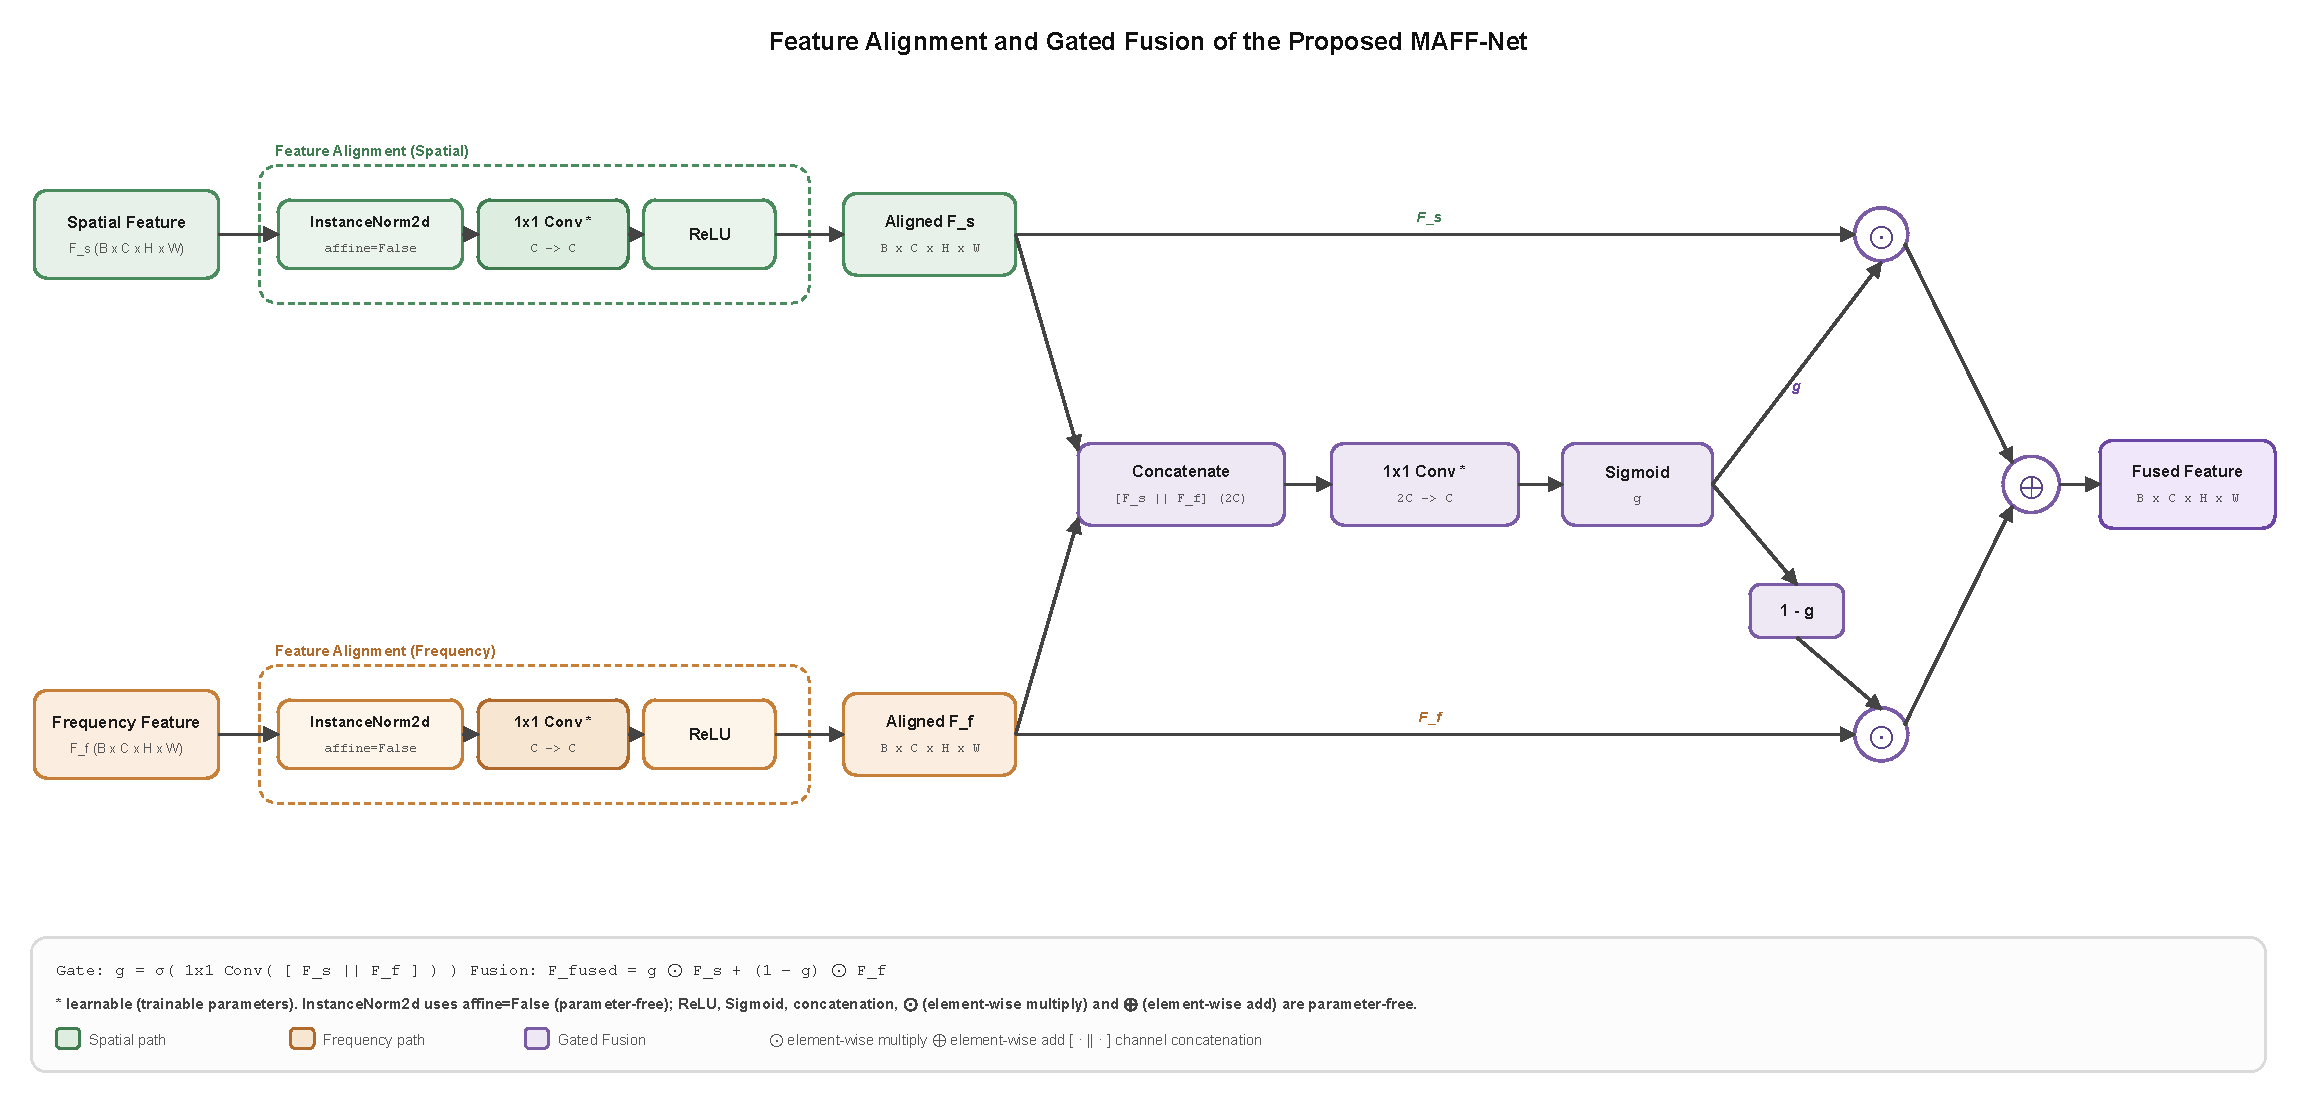
\includegraphics[width=\columnwidth]{Figure3_FeatureAlignment_GatedFusion.pdf}
\caption{Feature Alignment and Gated Fusion. The spatial and frequency features
are aligned independently by instance normalisation, a $1\times1$ convolution,
and a ReLU; the aligned features are then concatenated and passed through a
$1\times1$ convolution and a sigmoid to form a gate $g$, and the fused feature
is the convex combination $g\cdot F_s + (1-g)\cdot F_f$.}
\label{fig:fafusion}
\end{figure}

Within the dual-stream organisation of the Proposed MAFF-Net, the module is instantiated at each encoder scale and receives, at each scale, the two aligned representations produced by the Feature Alignment Module. It is therefore the stage at which the two parallel streams are brought back together: for every scale it consumes an aligned spatial representation and an aligned frequency representation and returns a single fused representation. These fused representations constitute the multi-scale features that the remainder of the network operates on; the deepest fused representation enters the decoder directly as its bottleneck input, while the three shallower fused representations are carried to the decoder through projected skip connections, so that the fused output of each scale contributes to the reconstruction of the segmentation map at the corresponding resolution. In this way the Gated Fusion Module occupies the position between alignment and decoding, converting the two aligned streams into the unified multi-scale representation on which the decoder depends.

With the two aligned streams combined into fused multi-scale representations, the network is ready to reconstruct the segmentation map from these representations. The decoding of the fused features, together with the auxiliary reconstruction branch that accompanies it, both of which are preserved from the Original MAFF-Net, is described in the following subsection.

\subsection{Decoder and Reconstruction Pathway}

Once the Gated Fusion Module has produced a fused representation at each encoder scale, a decoding stage transforms this set of fused multi-scale representations into a full-resolution segmentation prediction. The decoder is the final stage of the Proposed MAFF-Net, progressively resolving the fused features into a dense output at the resolution of the input image. Its decoding pathway is built on the design of the Original MAFF-Net and is not among the scientific contributions of this work; its function is to convert the outputs of the fusion pathway into a segmentation map.

Decoding proceeds hierarchically, from the coarsest fused representation to the finest. Beginning with the fused representation at the deepest scale, the decoder increases spatial resolution stage by stage; at each stage an upsampled higher-level feature is combined with a skip connection carrying information from the corresponding shallower scale, and the combined feature is refined before passing to the next stage. The finest stage refines the representation without a skip connection to complete the recovery of full resolution. Predictions are produced at multiple decoder stages: the highest-resolution one constitutes the segmentation output of the network, while the coarser stages provide additional multi-scale outputs. This coarse-to-fine organisation allows the decoder to recover the overall lesion region at the deeper stages and to sharpen the prediction toward the boundary as resolution increases.

The fused representations produced by the Gated Fusion Module differ from the features a conventional decoder would ordinarily receive, so the decoding pathway is adjusted to accept them: the skip connections entering the decoder are formed by applying a projection to the fused representations before they are combined with the upsampled decoder features, routing the dual-stream outputs into the decoder in a consistent form. This projection and routing are architectural adaptations required to accommodate the fused multi-scale representations; they are engineering adjustments that make the fusion pathway and the decoder compatible, not scientific contributions; the contributions of this work remain the Frequency Branch, the Feature Alignment Module, and the Gated Fusion Module, together with the supervision strategy described next, around which the decoding pathway is adapted.

Alongside the segmentation decoder, an auxiliary reconstruction branch operates on the same fused multi-scale representations and produces an image-sized reconstruction of the input. This provides an auxiliary reconstruction signal that supports training by encouraging the fused representations to retain information about the input. Like the decoder, it follows the design of the Original MAFF-Net, adapted to consume the fused representations rather than reproduced unchanged, and is likewise not claimed as a contribution. The decoder and the reconstruction branch thus draw on the same fused representations for two purposes: the decoder yields the lesion prediction, and the reconstruction branch yields an auxiliary output that regularises the shared representations during training.

The decoder and the reconstruction branch together determine the outputs of the network --- the multi-scale segmentation predictions and the auxiliary reconstruction --- but they do not by themselves specify how those outputs are supervised. The manner in which the multi-scale predictions and the reconstruction are used during training, and in particular the boundary-centric strategy that forms part of the training objective, is the subject of the following subsection on Boundary-centric Dual Supervision.

\subsection{Boundary-centric Dual Supervision}

The primary training signal for the Proposed MAFF-Net is a region-based segmentation objective that measures the agreement between the predicted and reference lesion regions. Such objectives recover the overall extent of a lesion effectively but are comparatively insensitive to errors confined to the boundary, because boundary pixels are few relative to the lesion interior and a small displacement of the contour changes the region-overlap measure only marginally --- a limitation that is particularly consequential in dermoscopy, where margins are frequently diffuse, gradual, or irregular and the clinical value of a segmentation depends heavily on boundary fidelity. To address this without displacing the region objective, the Proposed MAFF-Net augments it with supervision that explicitly targets the lesion contour, referred to as Boundary-centric Dual Supervision. BcDS supplements, rather than replaces, the primary region objective, and comprises two complementary pathways: Boundary-aware Deep Supervision applied to the segmentation outputs, and Edge-weighted Reconstruction applied to the reconstruction branch.

Boundary-aware Deep Supervision acts on the predictions produced by the decoder. The decoder emits predictions at multiple stages under deep supervision, and BDS supervises them by comparing their boundary structure with that of the ground-truth mask, so that discrepancies at the lesion contour are penalised directly. In contrast to the region objective, which compares predicted and reference areas, BDS compares predicted and reference edges, directing learning specifically toward accurate margins rather than overall region agreement. Because it is applied to the same multi-scale predictions that the region objective supervises, BDS adds a contour-oriented signal at each supervised decoder stage while leaving the region objective intact.

Edge-weighted Reconstruction acts on the auxiliary reconstruction branch, whose image-sized reconstruction of the input serves during training as a regularising signal on the shared fused representations. EWR shapes this signal so that the reconstruction discrepancy is emphasised in the regions surrounding the lesion boundary and de-emphasised in the comparatively uniform interior, turning an otherwise region-agnostic reconstruction objective into a boundary-emphasised one. By concentrating the reconstruction pressure along the margins, it encourages the fused representations on which both the decoder and the reconstruction branch depend to retain the boundary-related information that the segmentation prediction requires, reinforcing boundary fidelity indirectly, through the representations, rather than by acting on the prediction itself.

The two pathways impose a shared boundary focus through different outputs of the network, and are complementary rather than duplicative: one supervises what the network predicts at the contour, while the other supervises how well the underlying representations preserve boundary content. Together they constitute the dual character of Boundary-centric Dual Supervision. Both are auxiliary to, and coherent with, the region segmentation objective, sharpening boundary delineation while that objective continues to govern the recovery of the overall lesion region.

Boundary-centric Dual Supervision therefore supervises the multi-scale segmentation predictions and the auxiliary reconstruction with a common emphasis on the lesion boundary, while the region objective remains the primary training signal. The precise formulation of the region objective, the two boundary-focused terms, and the manner in which they are combined into a single training objective is presented in the following subsection.

\subsection{Training Objective / Loss Formulation}

The Proposed MAFF-Net is trained by minimising a single composite objective that combines a primary region-segmentation term with the two auxiliary boundary-focused terms of Boundary-centric Dual Supervision. Let $x$ denote the input dermoscopic image with $C$ channels, $y \in \{0,1\}^{H \times W}$ the binary ground-truth lesion mask, and $p_i$, for $i = 1,\dots,N$ with $N = 4$, the segmentation predictions (as logits) produced at the decoder stages under deep supervision. The logistic sigmoid is written $\sigma(\cdot)$, and sums indexed by $u$ run over spatial locations.

The region term is built from two standard segmentation losses. The soft Dice loss measures the overlap between a predicted probability map and the ground-truth mask,
\begin{equation}
L_{\mathrm{Dice}}(p,y) = 1 - \frac{2\sum_{u}\sigma(p)_u\,y_u + s}{\sum_{u}\sigma(p)_u + \sum_{u}y_u + s}, \tag{1}
\label{eq:1}
\end{equation}
where $s$ is a small smoothing constant that keeps the expression well defined when the mask or prediction is empty. The binary cross-entropy loss, applied to the logits with a positive-class weight $\omega$, measures per-pixel classification agreement,
\begin{equation}
\begin{aligned}
L_{\mathrm{BCE}}(p,y)
&=
-\frac{1}{|\Omega|}
\sum_{u\in\Omega}
\Big[
\omega\,y_u\log\sigma(p)_u
\\
&\qquad
+
(1-y_u)\log\big(1-\sigma(p)_u\big)
\Big].
\end{aligned}
\label{eq:2}
\end{equation}
where $\Omega$ is the set of spatial locations and $\omega$ up-weights lesion (positive) pixels relative to background pixels to counteract class imbalance.

The region objective aggregates these two losses over the deep-supervision predictions: each of the $N$ decoder predictions is supervised with the sum of the Dice and cross-entropy losses, and the results are averaged uniformly,
\begin{equation}
L_{\mathrm{seg}} = \frac{1}{N}\sum_{i=1}^{N}\Big[L_{\mathrm{Dice}}(p_i,y) + L_{\mathrm{BCE}}(p_i,y)\Big]. \tag{3}
\label{eq:3}
\end{equation}
In this uniform average every prediction contributes equally, so the region objective supervises the coarse and fine decoder stages with the same weight.

Boundary-aware Deep Supervision compares the boundary structure of the predictions with that of the ground truth, using an edge operator $S(\cdot)$ that applies the horizontal and vertical Sobel filters $G_x$ and $G_y$, forms the gradient magnitude, and bounds it to the unit interval,
\begin{equation}
S(m) = \mathrm{clamp}\!\Big(\sqrt{(G_x * m)^2 + (G_y * m)^2 + \varepsilon},\,0,\,1\Big), \tag{4a}
\label{eq:4a}
\end{equation}
where $*$ denotes convolution and $\varepsilon$ is a small constant that keeps the gradient of the square root finite in flat regions. The Boundary-aware Deep Supervision loss is then the weighted average, over the deep-supervision predictions, of the discrepancy between the predicted and ground-truth edge maps,
\begin{equation}
L_{\mathrm{BDS}} = \frac{1}{\sum_{i}w_i}\sum_{i=1}^{N} w_i \,\big\lVert\, S\big(\tilde{\sigma}(p_i)\big) - S(y)\,\big\rVert_1, \tag{4b}
\label{eq:4b}
\end{equation}
where $\tilde{\sigma}(p_i)$ is a smoothed sigmoid prediction and $w_i$ are per-prediction weights. Unlike the uniform aggregation of Eq.~\eqref{eq:3}, Eq.~\eqref{eq:4b} weights the predictions, so the finest dominate the boundary term while the coarsest contributes only marginally.

The boundary term is introduced gradually rather than from the first iteration. Its weight follows a linear warm-up schedule,
\begin{equation}
\lambda_{B}(t) = \lambda_{\mathrm{bds}}\cdot\min\!\Big(1,\ \frac{t}{T_{\mathrm{warm}}}\Big), \tag{5}
\label{eq:5}
\end{equation}
where $t$ is the current epoch index, $T_{\mathrm{warm}}$ is the warm-up length, and $\lambda_{\mathrm{bds}}$ is the maximum boundary weight. According to Eq.~\eqref{eq:5}, the weight rises from zero to $\lambda_{\mathrm{bds}}$ over the first $T_{\mathrm{warm}}$ epochs and is constant thereafter, so the region objective governs early training and the boundary term is phased in once the predictions have stabilised.

Edge-weighted Reconstruction supervises the auxiliary reconstruction branch with a boundary-emphasised reconstruction error. A spatial weight map is derived from the ground-truth boundary, $M = 1 + \alpha\,B(y)$, where $B(y)$ is a boundary band obtained from $S(y)$ and $\alpha \ge 0$ controls the emphasis placed on boundary regions. Writing $r$ for the reconstruction mapped to the range of the input image, the loss is a normalised weighted mean-squared error,
\begin{equation}
L_{\mathrm{EWR}} = \frac{\sum_{u} M_u\,(r_u - x_u)^2}{C\sum_{u} M_u}. \tag{6}
\label{eq:6}
\end{equation}
Because $M$ exceeds unity along the lesion boundary and equals unity elsewhere, Eq.~\eqref{eq:6} concentrates the reconstruction pressure on the boundary while normalising by the total weight and the number of channels $C$.

The complete training objective is the weighted sum of the region term and the two boundary terms,
\begin{equation}
L = L_{\mathrm{seg}} + \lambda_{B}(t)\,L_{\mathrm{BDS}} + \lambda_{\mathrm{ewr}}\,L_{\mathrm{EWR}}, \tag{7}
\label{eq:7}
\end{equation}
where $\lambda_{\mathrm{ewr}}$ is the reconstruction weight. In the implemented configuration, the region objective carries unit weight and is the dominant term, with $\lambda_{\mathrm{bds}} = 0.05$ and $\lambda_{\mathrm{ewr}} = 0.05$; the remaining constants are $\omega = 2$, $\alpha = 3$, $T_{\mathrm{warm}} = 5$, and per-prediction weights $w = (1, 1, 1, 0.01)$, with $s$ and $\varepsilon$ set to small fixed values.

The objective in Eq.~\eqref{eq:7} is minimised over the trainable parameters --- the fusion-pathway modules, the decoder, the segmentation heads, and the auxiliary reconstruction branch --- while the encoder remains frozen. Optimisation uses the AdamW optimiser with decoupled weight decay, a learning rate decayed linearly to zero over training, and gradient-norm clipping; training uses mixed-precision autocasting, and the model evaluated is the one with the best validation Dice score. Having specified the training objective, the following section describes the datasets, implementation, and evaluation protocol.
